\section{State redistribution in one dimension} \label{sec:srd1d}
We illustrate the state redistribution method on a simple example to gain some intuition in one dimension.  We solve the linear advection equation
\begin{equation}\label{eq:hpde}
u_t + au_x = 0
\end{equation}
on the nonuniform grid, called the base grid, shown in Figure \ref{fig:ng}, where $a > 0$.
Consider seven cells of this nonuniform grid, of which five cells (indexed by $-3$, $-2$, $0$, $2$, $3$) are large with size $h$ and the remaining two cells (indexed by $-1$ and $1$) are small with size $\alpha h$, where $0<\alpha \leq 1$.


We discretize \eqref{eq:hpde} using a first order upwind finite volume method.  After one forward Euler time step, the numerical solution is given by
\begin{equation}\label{eq:unstable1d}
\widehat{U}_i = U^n_i - \lambda_i(U^n_i -U^n_{i-1}),
\end{equation}
where $U^n_i$ is the solution average on cell $i$ at time step $t^n$, and the Courant number is $\lambda_i = a\Delta t / h_i$, with $h_i = h$ when $i \neq -1,1$ and $h_i = \alpha h$ for $i = -1,1$.  
%The update $\widehat{U}_i$ in \eqref{eq:unstable1d} is stable for $0\leq \lambda_i \leq 1$.
%On the small cells, we have
%\begin{equation}\label{eq:unstable1d+B}
%\widehat{U}_i = U^n_i - \frac{\lambda}{\alpha}(U^n_i -U^n_{i-1}) \text{ for } i = -1,1,
%\end{equation}
%where $0 < \alpha \ll 1$ and $\widehat{U}_i$ is a stable solution update for $0 \leq \lambda \leq \alpha$.  
We call the finite volume method in \eqref{eq:unstable1d} the base scheme.  
The maximum stable time step of the base finite volume scheme on this grid would be $\Delta t \leq \alpha h/a$, i.e., it can be arbitrarily small since $0 < \alpha \leq 1$.  

In this work, we propose an approach, called ``state redistribution", to relax this overly restrictive maximum stable time step.
The state redistribution method is a post-processing procedure that acts on the base scheme and stabilizes $\widehat{U}_i$ in a conservative manner.  This is done by temporarily merging cells of the grid into larger, possibly overlapping, neighborhoods and recombining the solution averages on these neighborhoods in a particular fashion.
These merged cells are constructed once during a mesh preprocessing stage before execution of the iterative portion of the finite volume solver.

\begin{figure}
		\centering
		\subfloat[Nonuniform base grid with two small cells $-1$ and $1$.  The small and large cell sizes are $\alpha h$ ($0<\alpha \ll 1$), and $h$, respectively.]{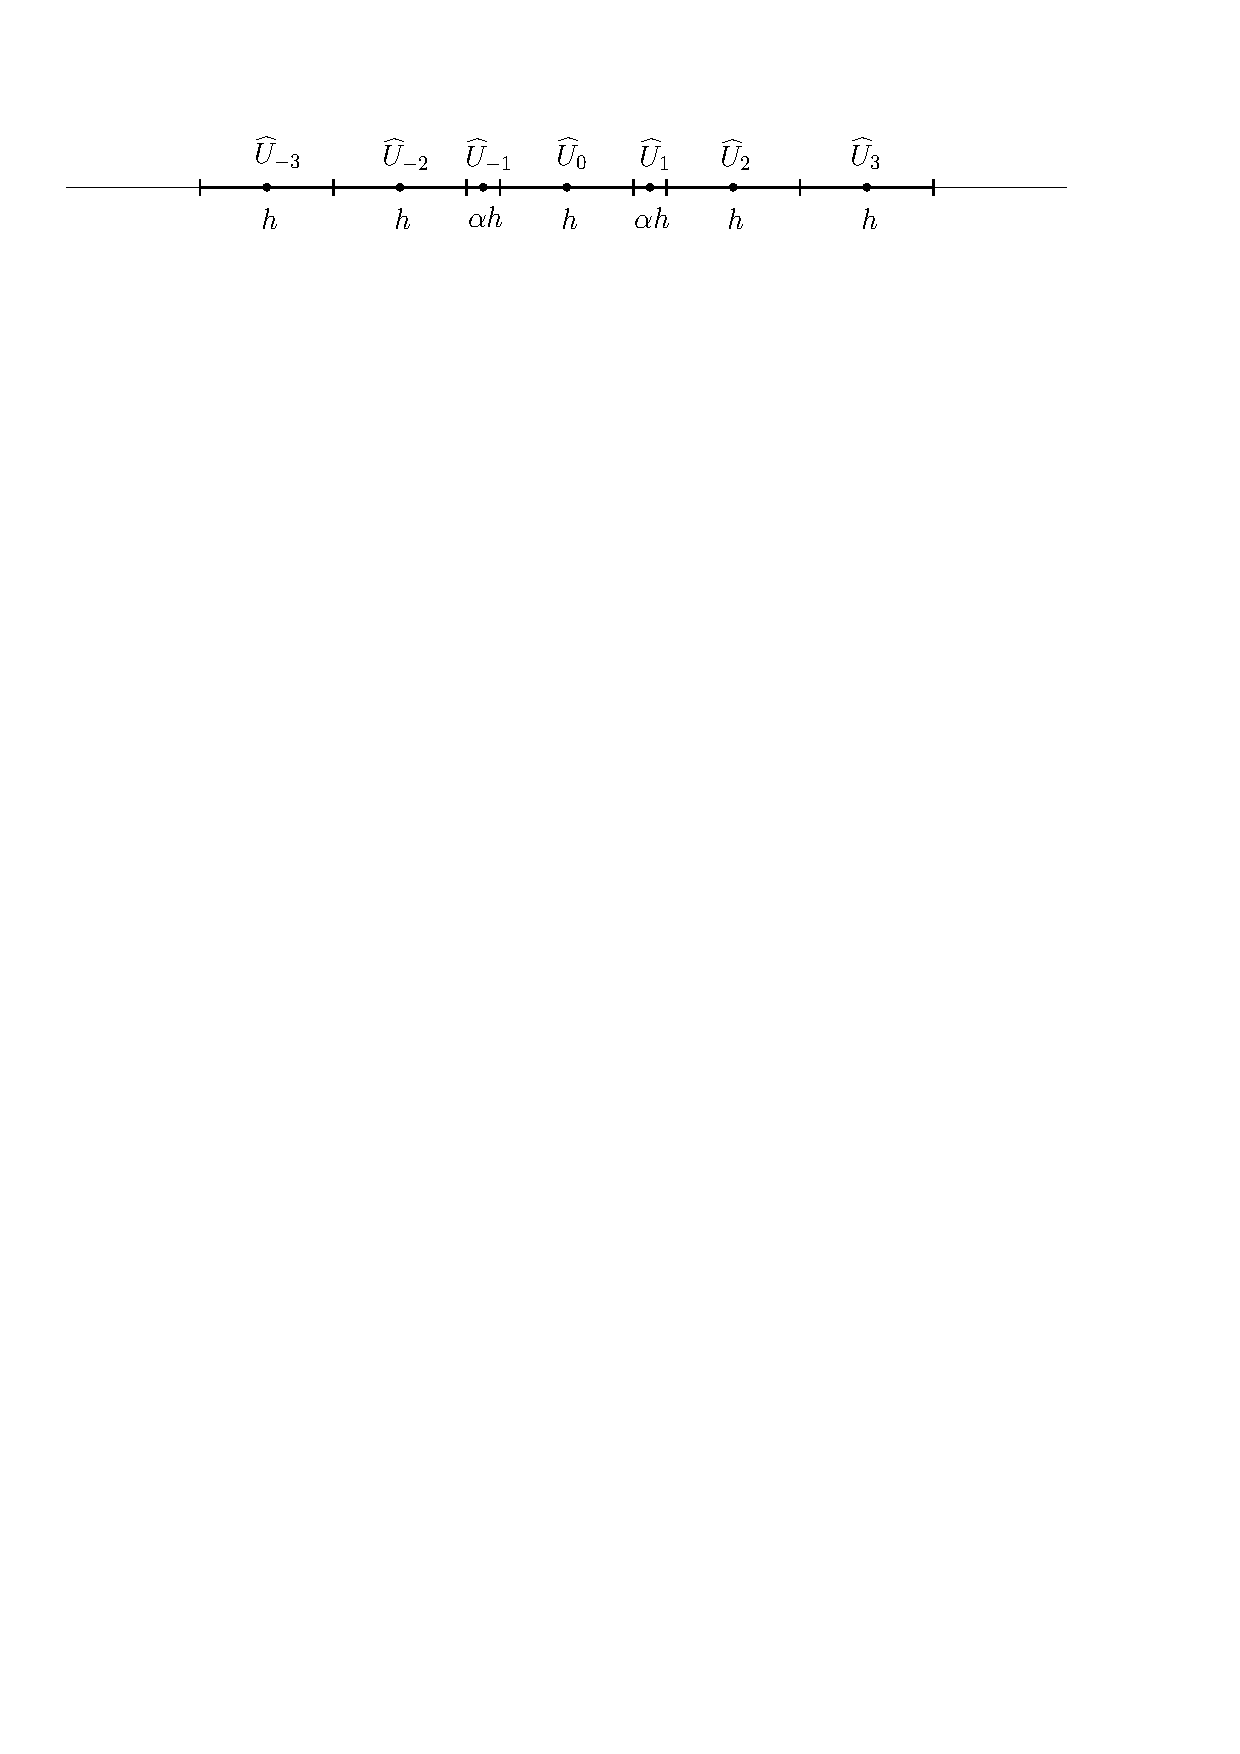
\includegraphics[width=0.75\linewidth]{figs/overlapping.pdf} \label{fig:ng}}
		\hfill
		\subfloat[Each blue arrow indicates the merging neighborhoods associated to the large cells $-3$, $-2$, $0$, $2$, and $3$.  The number above each blue arrow is the neighborhood index.
		The red arrow corresponds to the neighborhood of small cells $-1$ and $1$, where the number below each red arrow is the neighborhood index.
%		The numbers in red and blue indicate the cells contained in the associated neighborhoods.
		]{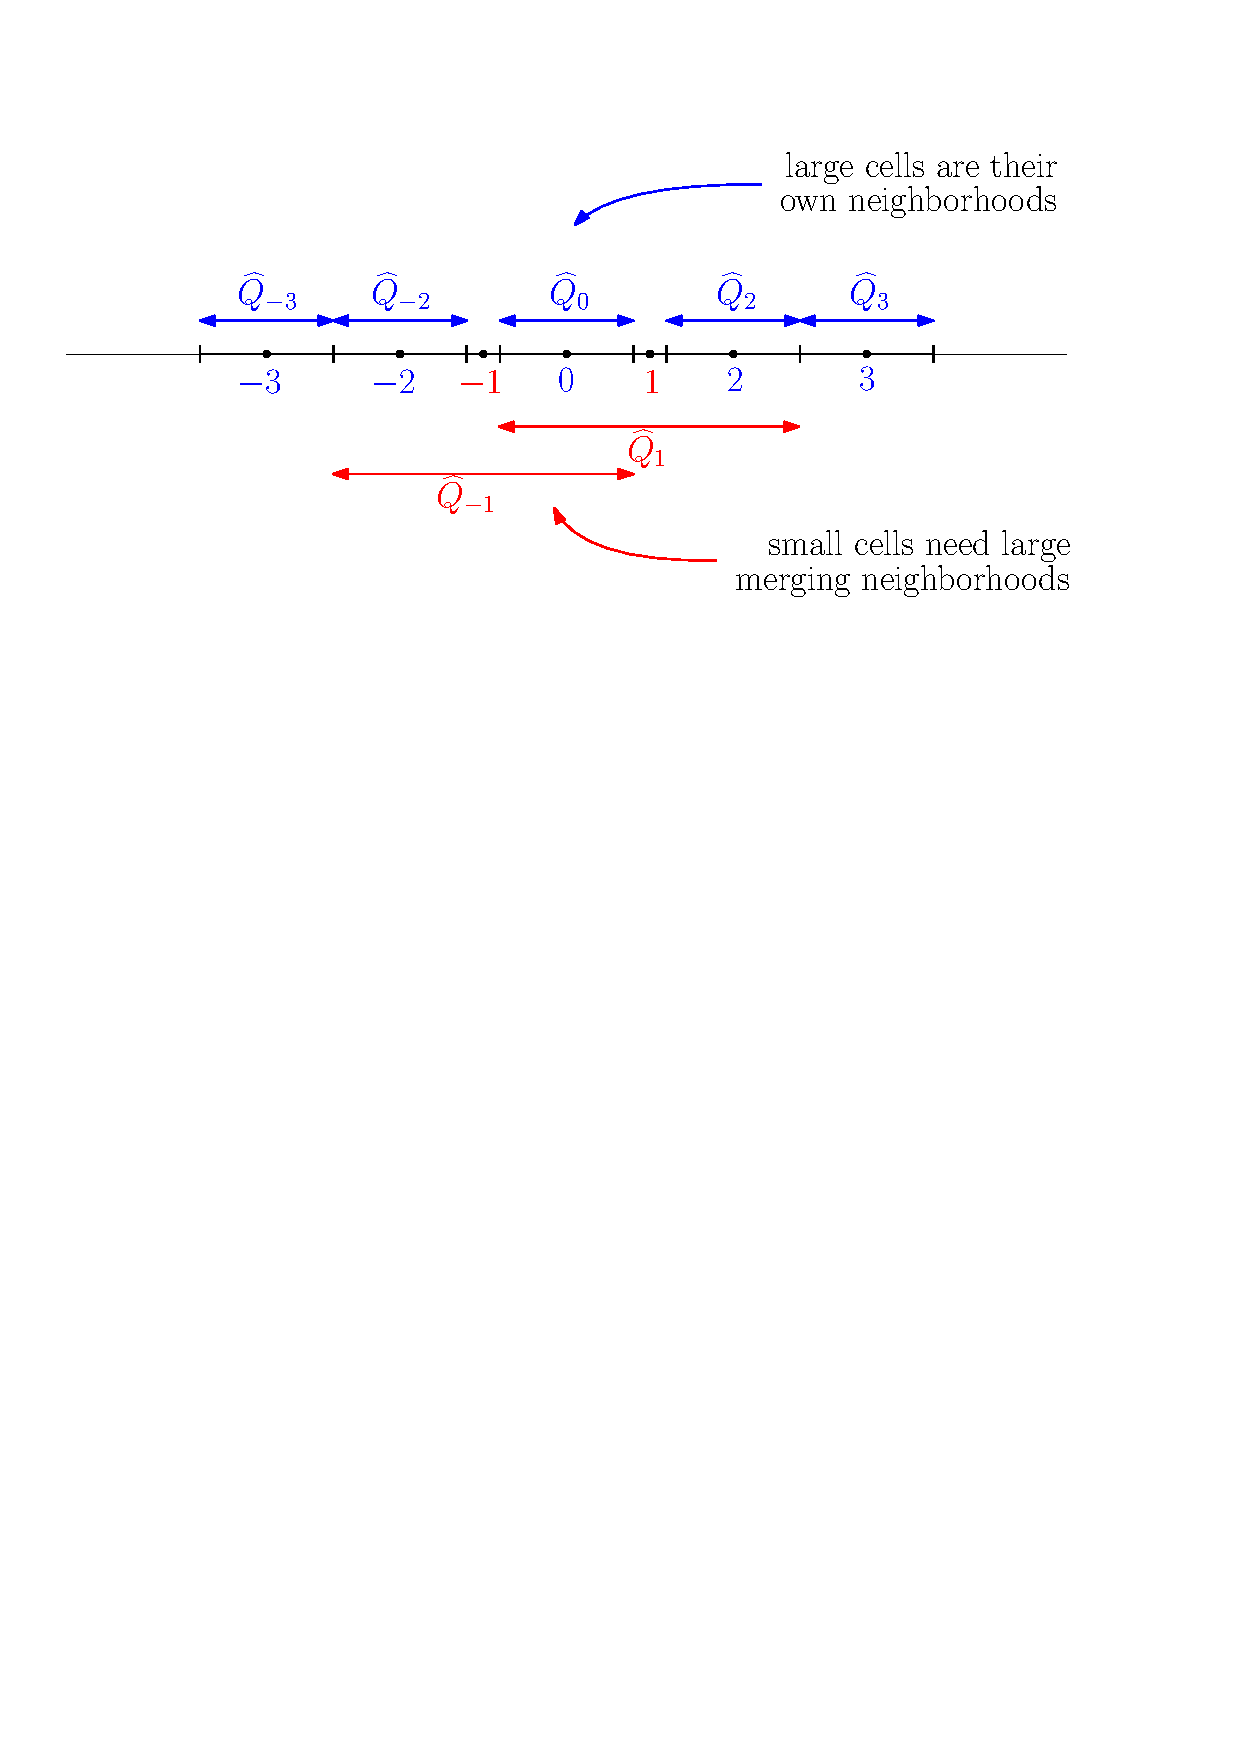
\includegraphics[width=0.75\linewidth]{figs/overlapping1.pdf} \label{fig:mn1}}
		\hfill
%		\subfloat[The number of overlapping neighborhoods on each cell in the base grid.]{\includegraphics[width=0.75\linewidth]{figs/overlapping3.pdf} \label{fig:mn3}}
		\caption{\sf Model problem in one space dimension. The small
			cells have size $\alpha h$ in a mesh with regular mesh width $h$.}
		\label{fig:modelProblem1}
\end{figure}

\subsubsection*{State redistribution preprocessing}
Each cell in the base grid (both large and small) has a merging neighborhood associated to it, i.e., each cell finds a set of neighbors with which to merge temporarily.
Neighborhoods share the same index as the cell that generated it.
%The merging neighborhood associated to cell $i$ is called $M_i$. 
Small cells merge with their neighbors until the volume of the merging neighborhood is greater than, e.g., half the large cell size $h/2$.
This is illustrated by the red arrows in Figure \ref{fig:mn1} where the merging neighborhood of small cell $-1$ consists of cells $-2$, $-1$, and $0$ and the merging neighborhood of small cell 1 consists of cells $0$, $1$, and $2$. 
A large cell does not need to merge with neighbors (since $h > h/2$), thus its merging neighborhood is only composed of itself.  This is illustrated by the blue arrows in Figure \ref{fig:mn1}, where the merging neighborhood of, e.g., large cell $-3$ is composed only of itself.
Finally, each cell in the base grid counts the number of neighborhoods that overlap it, e.g., cell $-2$ is overlapped by two neighborhoods, indexed by $-1$ and $-2$.

%\subsubsection*{Overlap count}
%Each cell in the base grid counts the number of neighborhoods that overlap it, as illustrated in Figure \ref{fig:mn3}.  
%%The overlap count associated to cell $i$ is called $N_i$.
%For example, cell $0$ is overlapped by three merging neighborhoods, i.e., the neighborhoods associated to cells $-1$, $0$,  and $1$.
\subsubsection*{State redistribution postprocessing}
Using the above information, we can now stabilize \eqref{eq:unstable1d} using the state redistribution method on the grid in Figure \ref{fig:modelProblem1}.  
On each merging neighborhood, we compute a weighted solution average, $\widehat Q_i$, where $i$ is the index of the merging neighborhood. 
$\widehat Q_i$ is computed by convex combination of the averages $\widehat{U}_i$ on cells contained in the merging neighborhood. 
On merging neighborhood $-1$, the weighted solution average is
\begin{equation}\label{eq:neigh2}
\widehat{Q}_{-1} = \frac{1}{\underbrace{h/2 + \alpha h + h/3}_{\text{weighted volume}}}\biggr( \underbrace{\frac{h}{2} \widehat{U}_{-2} + \alpha h \widehat{U}_{-1} + \frac{h}{3}\widehat{U}_{0}}_{\text{weighted mass}} \biggr).
\end{equation}
Note that in the above formula for the weighted solution average, we divide cell volume by the number of neighborhoods that overlap the associated cell in the base grid. 
For example, the multiplier in front of $\widehat{U}_{-2}$ is $\frac{h}{2}$ since there are two neighborhoods that overlap cell $-2$, i.e., cell $-2$ is overlapped by neighborhoods $-1$ and $-2$.  
Similarly, the multiplier in front of $\widehat{U}_{-1}$ is $\alpha h$ since there is only one neighborhood that overlaps cell $-1$, i.e. cell $-1$ is overlapped by neighborhood $-1$.
Finally, the multiplier in front of $\widehat{U}_{0}$ is $\frac{h}{3}$ since there are three neighborhoods that overlap cell $0$, i.e., cell $0$ is overlapped by neighborhoods $-1$, $1$, and $0$.
These multipliers are then divided by $(h/2 + \alpha h + h/3)$ since $\widehat{Q}_{-1} $ must be a convex combination of $\widehat{U}_{-2}$, $\widehat{U}_{-1}$, and $\widehat{U}_{0}$.
The weighted solution average on merging neighborhood $1$ is similarly defined as
\begin{equation}\label{eq:neigh3}
\widehat{Q}_{1} = \frac{1}{h/2 + \alpha h + h/3}\left( \frac{h}{2} \widehat{U}_{2} + \alpha h \widehat{U}_{1} + \frac{h}{3}\widehat{U}_{0} \right).
\end{equation}
The weighted solution averages on merging neighborhoods that contain only one cell are simply 
\begin{equation}\label{eq:neigh1}
\widehat{Q}_i = \widehat{U}_i \text{ for } i = -3,-2,0,2,3.
\end{equation}
%The stabilized solution average at $t^{n+1}$, $U^{n+1}_i$ on the base grid can then be defined in terms of the weighted solution average on neighborhoods, $\widehat{Q}_{i}$.  

The stabilized solution average at time $t^{n+1}$ on a cell in the base grid is then given by the average of all the weighted neighborhood averages that overlap it.  That is, on the cell overlapped by three neighborhoods, we have
\begin{equation} \label{eq:threeneigh}
U^{n+1}_{0} = \frac{1}{3}(\widehat{Q}_{-1}+\widehat{Q}_{0}+\widehat{Q}_{1}).
\end{equation}
On cells overlapped by two neighborhoods, we have
\begin{equation} \label{eq:twoneigh}
U^{n+1}_{-2} = \frac{1}{2}(\widehat{Q}_{-1}+\widehat{Q}_{-2}) \text{ and } U^{n+1}_{2} = \frac{1}{2}(\widehat{Q}_{1}+\widehat{Q}_{2}).
\end{equation}
Finally, on cells overlapped by only one neighborhood,  we have
\begin{equation} \label{eq:oneneigh}
	U^{n+1}_i = \widehat{Q}_i \text{ for } i = -3,-1,1,3.
\end{equation}
%On cells overlapped by two neighborhoods, we have
%\begin{equation} \label{eq:twoneigh}
%U^{n+1}_{-2} = \frac{1}{2}(\widehat{Q}_{-1}+\widehat{Q}_{-2}) \text{ and } U^{n+1}_{2} = \frac{1}{2}(\widehat{Q}_{1}+\widehat{Q}_{2}).
%\end{equation}
%Finally, on the cell overlapped by three neighborhoods, we have
%\begin{equation} \label{eq:threeneigh}
%U^{n+1}_{0} = \frac{1}{3}(\widehat{Q}_{-1}+\widehat{Q}_{0}+\widehat{Q}_{1}).
%\end{equation}
Writing the solution stabilized by state redistribution on the small cells at $t^{n+1}$ in terms of the solution averages at $t^{n}$, we have
\begin{equation}
\begin{aligned}
U^{n+1}_{-1} &= \frac{2-2\lambda}{5+6\alpha}U^n_0 + \frac{6\alpha - 4 \lambda}{5+6\alpha}U^n_{i-1}+ \frac{3\lambda + 3}{5+6\alpha}U^n_{i-2}+\frac{3\lambda }{5+6\alpha}U^n_{i-3}, \\
U^{n+1}_{1} &= \frac{2+4\lambda}{5+6\alpha}U^n_0 + \frac{6\alpha - 3 \lambda}{5+6\alpha}U^n_{i+1}+ \frac{3-3\lambda}{5+6\alpha}U^n_{i+2}+\frac{2\lambda }{5+6\alpha}U^n_{i-1}.
\end{aligned} \label{eq:finalupdate}
\end{equation}
Before application of the state redistribution method, the weights that multiply the solution averages at time $t^n$ in the base scheme \eqref{eq:unstable1d} become unbounded as $\alpha \rightarrow 0$.
However, now that the state redistribution is applied to the base scheme, this is no longer the case for the weights in \eqref{eq:finalupdate} as $\alpha \rightarrow 0$.  This hints at the stability of our modified scheme.  

The goal of the state redistribution method is to allow us to take time steps as if there were no small cells in the grid, that is, use $\Delta t = h / a$.  Using this time step, the multipliers of $U^n_{i-1}$ and $U^n_{i+1}$ in \eqref{eq:finalupdate} are negative when $\alpha$ is small enough.  This means that our scheme is not monotone and thus not total variation diminishing.  However, we note that this is also the case for other popular small cell stabilization schemes such as, e.g., flux redistribution.

\subsubsection*{Conservation}
We now show that our modified scheme \eqref{eq:threeneigh}, \eqref{eq:twoneigh}, \eqref{eq:oneneigh} conserves mass.
%, i.e., the total mass of the numerical solution before and after state redistribution is the same.  
For the portion of the grid in question, the total mass after state redistribution is
\begin{equation}\label{eq:tm1}
	\sum_{i} h_i U^{n+1}_i  = h U^{n+1}_{-3} + h U^{n+1}_{-2} + \alpha h U^{n+1}_{-1} +h U^{n+1}_0+\alpha h U^{n+1}_{1} + h U^{n+1}_{2} + h U^{n+1}_{3},
\end{equation}
where $h_i$ is the local cell size, i.e., $h_i = \alpha h$ for $i \neq -1,1$ and $h_i = h$ otherwise.
Substituting expressions for the final update \eqref{eq:oneneigh}, \eqref{eq:twoneigh}, \eqref{eq:threeneigh} into \eqref{eq:tm1}, we obtain
\begin{equation}\label{eq:tm2}
\begin{aligned}
\sum_{i} h_i U^{n+1}_i  &= h \widehat{Q}_{-3} + \frac{h}{2}(\widehat{Q}_{-1}+\widehat{Q}_{-2}) \\
&+ \alpha h \widehat{Q}_{-1} +h \frac{1}{3}(\widehat{Q}_{-1}+\widehat{Q}_{0}+\widehat{Q}_{1})+\alpha h \widehat{Q}_{1} \\
&+ h \frac{1}{2}(\widehat{Q}_{1}+\widehat{Q}_{2}) + h \widehat{Q}_{3}.
\end{aligned}
\end{equation}
Grouping terms in \eqref{eq:tm2}, we have
\begin{equation}\label{eq:tm3}
\begin{aligned}
\sum_{i} h_i U^{n+1}_i  &= h \widehat{Q}_{-3} + \frac{h}{2}\widehat{Q}_{-2} \\
&+ \left(\frac{h}{2}+\alpha h + \frac{h}{3}\right) \widehat{Q}_{-1} + \frac{h}{3} \widehat{Q}_0 + \left(\frac{h}{2}+\alpha h + \frac{h}{3}\right) \widehat{Q}_{1} \\
&+ \frac{h}{2}\widehat{Q}_{2} + h \widehat{Q}_3.
\end{aligned}
\end{equation}
Substituting the expressions for the neighborhood averages \eqref{eq:neigh1}, \eqref{eq:neigh2}, \eqref{eq:neigh3} into \eqref{eq:tm3}, we obtain
\begin{equation}\label{eq:tm4}
\begin{aligned}
\sum_{i} h_i U^{n+1}_i  &= h \widehat{U}_{-3} + \frac{h}{2}\widehat{U}_{-2} \\
&+ \left(\frac{h}{2} \widehat{U}_{-2} + \alpha h \widehat{U}_{-1} + \frac{h}{3}\widehat{U}_{0}\right) + \frac{h}{3} \widehat{U}_0 + \left(\frac{h}{2} \widehat{U}_{2} + \alpha h \widehat{U}_{1} + \frac{h}{3}\widehat{U}_{0}\right) \\
&+ \frac{h}{2}\widehat{U}_{2} + h \widehat{U}_3.
\end{aligned}
\end{equation}
Simplifying \eqref{eq:tm4}, the mass after state redistribution becomes
\begin{equation}\label{eq:tm5}
\begin{aligned}
\sum_{i} h_i U^{n+1}_i  &= h \widehat{U}_{-3} + h \widehat{U}_{-2} + \alpha h \widehat{U}_{-1} +h \widehat{U}_0+\alpha h \widehat{U}_{1} + h \widehat{U}_{2} + h \widehat{U}_{3},\\
&= \sum_{i} h_i \widehat{U}_i.
\end{aligned}
\end{equation}
Thus, the mass on the grid before and after state redistribution does not change.
Since the base scheme \eqref{eq:unstable1d} is conservative, it follows from \eqref{eq:tm5} that our modified scheme \eqref{eq:threeneigh}, \eqref{eq:twoneigh}, \eqref{eq:oneneigh} conserves mass.
%, our modified scheme \eqref{eq:threeneigh}, \eqref{eq:twoneigh}, \eqref{eq:oneneigh} is conservative.  
%Thus, the base scheme coupled with the state redistribution method is conservative.  




The stabilized finite volume method \eqref{eq:threeneigh}, \eqref{eq:twoneigh}, \eqref{eq:oneneigh} is first order accurate in space and time.  In this work, we provide a framework to generalize the state redistribution method to two dimensional cut cell grids and to arbitrarily high-order accuracy in space and time.
We will demonstrate on cut cell grids that the above stabilization procedure solves the small cell problem, i.e., that the maximum stable time step is no longer restricted by the small cells, and that the state redistribution method is conservative, i.e.,
$$
 \sum_{i}h_i U^{n+1} = \sum_{i}h_i \widehat{U}_i.
$$



In the next section  we discuss the base finite volume schemes that will be stabilized by state redistribution.

\textit{Note}: the key difference between state redistribution and cell merging is that state redistribution supports overlapping neighborhoods and cell merging does not. 
As a result, cell merging can be difficult to implement in a robust manner in three dimensions since there are many different, possibly incompatible ways to create non-overlapping merging neighborhoods.
State redistribution does not suffer from this difficulty, and its extension to three dimensions is straightforward.
%The SRD algorithm in two space dimensions will be presented in Section
%\ref{sec:srdAlg}.
%Some theoretical results using one-dimensional model problems are in Section \ref{sec:theory}. 
%For simplicity we present the second order accurate version first.
%The more general higher order extension is described in Appendix \ref{sec:ho}.
%Section \ref{sec:compResults} shows computational results for both smooth
%problems and shocked flow for both linear advection and the Euler equations.  We conclude in section \ref{sec:conc}.


%Contrast these weighted solution averages, with the standard solution average on merging neighborhood $-1$
%$$
% \frac{h}{h + \alpha h + h} \widehat{U}_{-2} + \frac{\alpha h}{h + \alpha h + h} \widehat{U}_{-1} + \frac{h}{h + \alpha h + h}\widehat{U}_{0}
%$$
%and the standard solution average on merging neighborhood $1$ is
%$$
%\frac{h}{h + \alpha h + h} \widehat{U}_{2} + \frac{\alpha h}{h + \alpha h + h} \widehat{U}_{1} + \frac{h}{h + \alpha h + h}\widehat{U}_{0}.
%$$



%\subsubsection*{Weighted volume of merging neighborhood}
%Each merging neighborhood has an associated a weighted volume




%\begin{equation}
%	\widehat{V}_i = \sum_{i \in M_i} \frac{h}{den}
%\end{equation}

%\subsubsection*{Solution average on merging neighborhood}
%We compute a weighted solution average on each merging neighborhood, $M_i$, using the following formula
%\begin{equation}\label{eq:merging}
%	\widehat{Q}_{i} = 
%\end{equation}



%The merging cell consists consisting of the small cell $u_j$ and one or both of its neighbors so that it the merged cell is of sufficient

%\begin{figure}
%	\subfloat[$50\times50$ grid and annulus domain.]{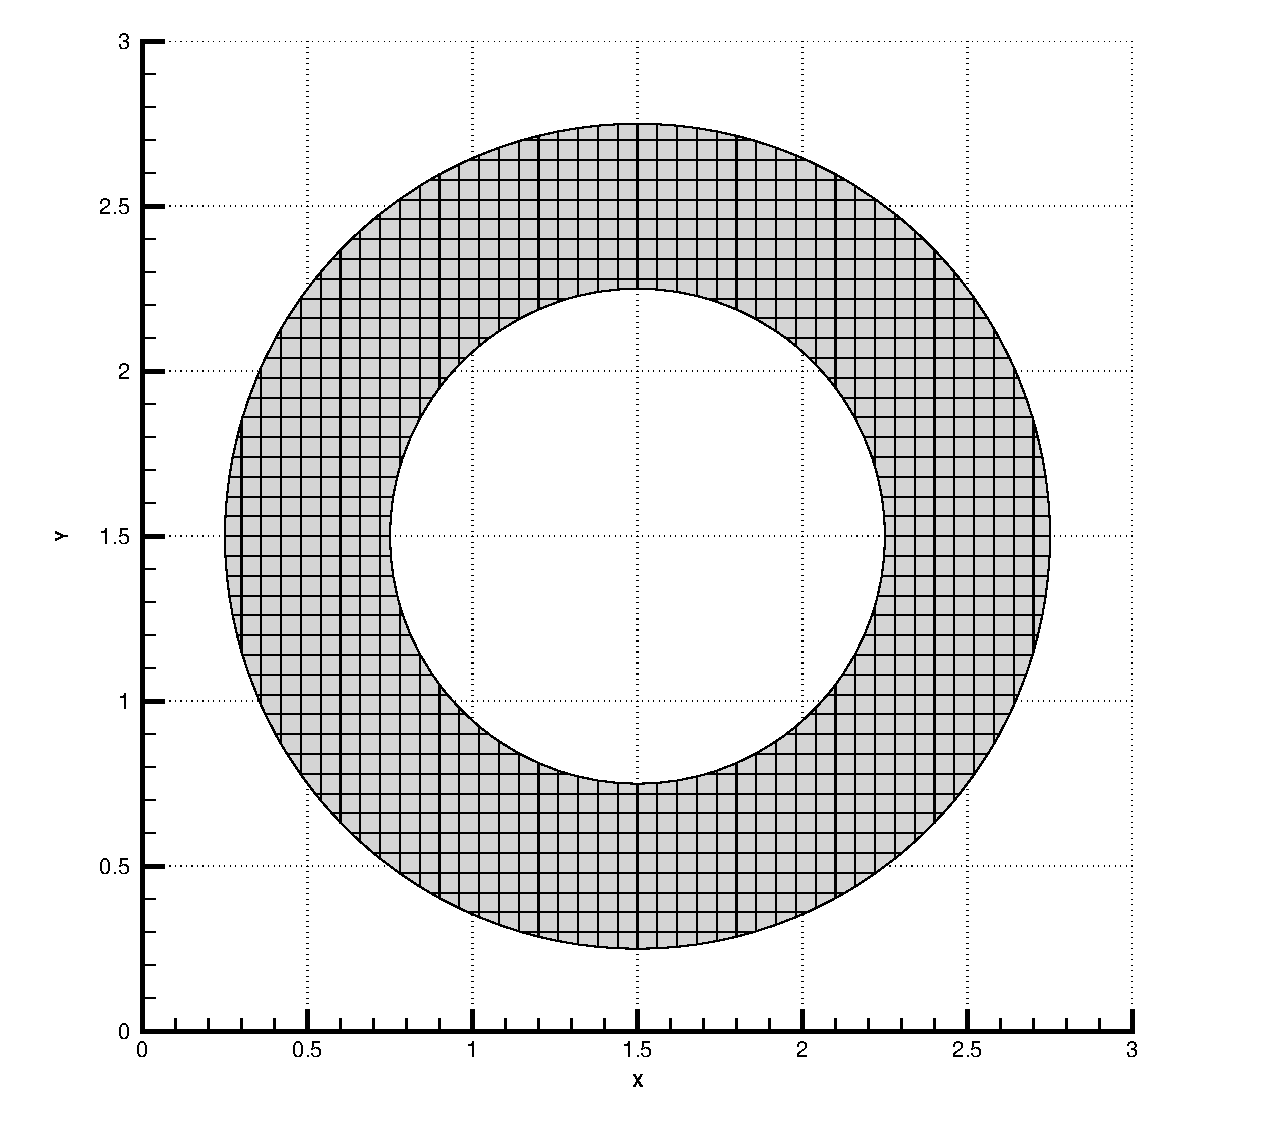
\includegraphics[width = 0.5\linewidth]{figs/rotatinghill_grid.eps} \label{fig:rotatinghillgrid}} 
%	\quad
%	\subfloat[Isolines of exact solution at the initial and final time. SHOW
%	COMPUTED SOLUTION TOO]{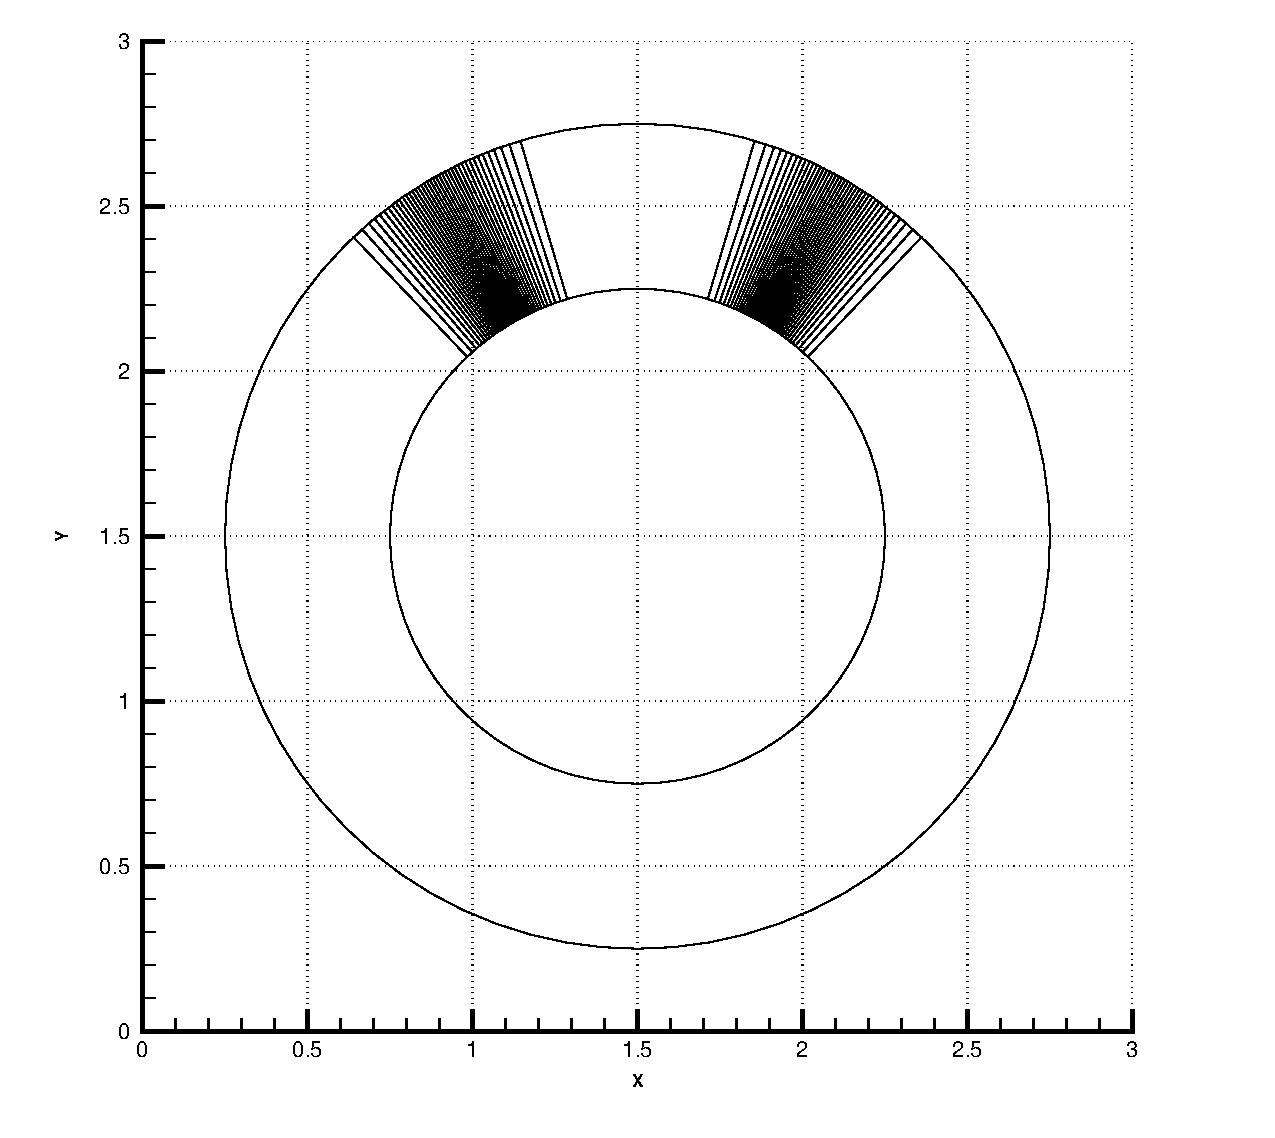
\includegraphics[width = 0.5\linewidth]{figs/rotatinghill_solution.eps}\label{fig:rotatinghillexactiso}}
%\end{figure}
%\begin{figure}
%	\begin{center}
%		%\vspace*{-.5in}
%		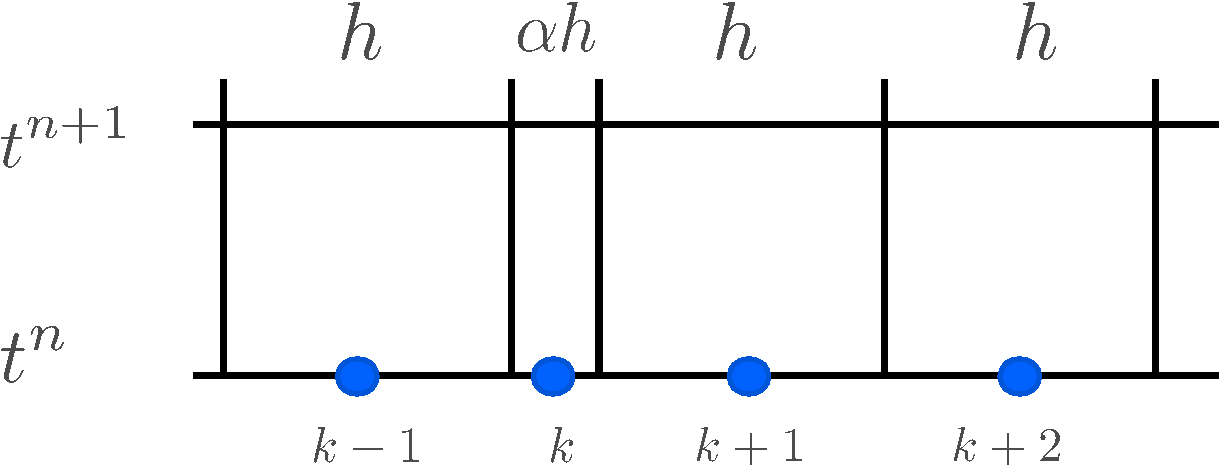
\includegraphics[height=1.3in]{figs/1dfig.pdf}
%		\caption{\sf Notation for model problem in one space dimension. The small
%			cell has size $\alpha h$ in a mesh with regular mesh width $h$.}
%		\label{fig:modelProblem1}
%	\end{center}
%\end{figure}


%To set the stage, notice that cell merging itself can
%be rewritten as a postprocessing step.
%\commentout{
%To take one step to update a finite volume approximation to
%$u_t + u_x = 0$ we do the following:
%\begin{itemize}
%\setlength\itemsep{.2in}
%\item
%{\bf Finite Volume Step}\\
%Take the usual finite volume step with fixed, regular  $\Delta t$ on all cells 
%including the small cell:
%\begin{equation}
%\bar{u}_j = u_j^n - \frac{\Delta t}{h_j} \; (f_{j+1/2} - f_{j-1/2} ), 
%\quad \forall j.
%\label{eqn:fvupdate}
%\end{equation}
%
%\item
%{\bf {\em Temporarily} Create Merged Cell}\\
%Temporarily create the {\em merged} cell $\overline{u_M}$ consisting of the small cell $u_j$ and one
%or both of its neighbors so that it the merged cell is of sufficient
%size (to be discussed later).  For simplicity here we will merge 
%only with the neighbor on the right,
%\begin{equation}
%\widehat{q_M} =  \frac{ h_k \bar{u}_k + h_{k+1} \bar{u}_{k+1} } {h_k +
%h_{k+1}} .
%\label{eqn:mergestep}
%\end{equation}
%
%\item
%{\bf Compute Merge Cell Gradient }\\
%There are several ways to do this. 
%Two simple possibilities are 
%\begin{equation}
%\nabla \widehat{u_M} = \frac{\bar{u}_{k+2} - \bar{u}_{k-1}} {x_{k+2}-x_{k-1}}
%\label{eqn:gradLim1}
%\end{equation}
%which does not use the merged cell,
%or
%\begin{equation}
%\nabla \widehat{u_M} = \frac{\bar{q}_{k+2} - \widehat{u_{M}}} {x_{k+2}-x_{M}}
%\label{eqn:gradLim2}
%\end{equation}
%which uses the merged cell, and $x_M$ is the centroid of the merged
%cell.
%The choice of gradient stencil will be studied later in section \ref{sec:srdAlg}.
%
%%Other more accurate alternatives exist, not all of which are stable.
%%It would be better to use smaller stencils, perhaps including $u_{k+1}$
%%or $\overline{u_M}$ itself.
%
%\item
%{\bf Redistribute Merged State to Cells Comprising Merged cell }\\
%Replace the provisional values computed in the cells comprising the
%merged cell with the merged solution reconstructed to the cell
%centroids:
%\begin{equation}
%\begin{split}
%u_k^{n+1} &= \widehat{u_M} +  (x_k - x_M) \nabla \widehat{u_M}\\
%u_{k+1}^{n+1} &= \widehat{u_M} +  (x_{k+1} - x_M) \nabla \widehat{u_M}
%\end{split}
%\end{equation}
%\end{itemize}
%}
%First update cells $k$ and $k+1$, shown in Figure \ref{fig:modelProblem1},  using a 
%standard finite volume scheme on all cells:
%\begin{equation}
%\bar{u}_j = u_j^n - \frac{\Delta t}{h_j} \; (f_{j+1/2} - f_{j-1/2} ), 
%\quad \forall j.
%\label{eqn:fvupdate}
%\end{equation}
%Next form the merged cell
%\begin{equation}
%\widehat{q_M} =  \frac{ h_k \bar{u}_k + h_{k+1} \bar{u}_{k+1} } {h_k +
%h_{k+1}} .
%\label{eqn:mergestep}
%\end{equation}
%which works out to
%\begin{equation}
%\widehat{q_M} = \widehat{q_M}^n - 
%\frac{\Delta t}{h_k + h_{k+1}} (f_{k+3/2} - f_{k-1/2})
%\end{equation}
%For the simplest first order version, we simply set
%\begin{equation}
%u_k^{n+1} = u_{k+1}^{n+1} = \widehat{q_M} 
%\label{eqn:finalstep}
%\end{equation}
%Recognizing that $h_k+h_{k+1}$ is the merged cell volume makes 
%clear the relationship to cell merging.
%The final update step \eqref{eqn:finalstep} is replaced by 
%\begin{equation}
%\begin{split}
%u_k^{n+1} &= \widehat{q_M} +  (x_k - \widehat{x}_M) \,\,  \widehat{\sigma_M}\\
%u_{k+1}^{n+1} &= \widehat{q_M} +  (x_{k+1} - \widehat{x}_M) \,  \widehat{\sigma_M}
%\end{split}
%\end{equation}
%where $\widehat{\sigma_M}$ is a reconstructed slope on the merged cell.
%The state redistribution method is linearity preserving when the base finite volume scheme and the reconstructed slope on merged cells $\widehat{\sigma_M}$ are accurate enough.
%By using a polynomial of degree $p>1$ and
%including more neighbors in the
%redistribution (on top of a more accurate finite volume scheme for the
%entire mesh),
%we have a path to higher order accuracy.
%The method is also conservative since the mass of the merged cell equals the 
%mass of the two cells comprising it.



%The choice of merging neighborhoods and gradients is what makes up the
%specifics of SRD in two space dimensions. Furthermore, it can happen
%that a cell has more than one neighborhood with
%which it should merge. This is what often causes complications in cell
%merging algorithms. In SRD, we will simply use all such values appropriately
%weighted.
%
%In the next section  we first discuss the finite volume schemes to which SRD will
%be applied.
%The SRD algorithm in two space dimensions will be presented in section
%\ref{sec:srdAlg}.
%For simplicity we present the second order accurate version first.
%The more general higher order extension is described in 
%section \ref{sec:ho}.
%Some theoretical results using one-dimensional model problems are in
%section \ref{sec:theory}. 
%Section \ref{sec:compResults} shows computational results for both smooth
%problems and shocked flow for both linear advection and the Euler equations.  We conclude in section \ref{sec:conc}.